%!TEX root = main.tex

本文关注从无标记单眼RGB图像序列恢复3D全身人体姿势的挑战。我们工作的潜在应用包括人机交互,监控,康复,体育,视频浏览和索引以及虚拟现实。
此任务的典型解决方案包括带有多个摄像头和反射标记和深度传感器的动作捕捉(MoCap)系统, 例如, Microsoft Kinect \cite{kinect}. 这些技术需要定制设备,仅限于受限环境中的应用程序,并且不能应用于归档RGB图像或视频。 本文通过使用单个摄像头并避免使用标记来解决姿势恢复挑战:
直接从2D外观转到3D几何体。
 

从几何的角度来看,从单目图片恢复3D骨架姿态本质上是有歧义的\cite{lee1985determination}。相当多的工作通过骨架约束\cite{taylor2000reconstruction}, 低阶先验\cite{bregler2000recovering}, 稀疏表达 \cite{ramakrishna2012reconstructing}, 或者用身体模型跟踪从2D的对应关系重建3D人体姿势 \cite{bregler1998tracking}。这些方法通常假设提供2D对应关系,或者需要基于低级图像特征仔细跟踪帧到帧之间的关系。 由于人体外观(例如,衣服,体形和照明),相机的变换视角以及由于自遮挡和外部实体的遮挡,导致的人体可见性的巨大变化,使得寻找2D的对应关系比较困难。

在2D的姿态估计中,结合2D的身体部位模型与变形信息的方法取得了显著的成功,例如 \cite{yang2011articulated,andriluka20142d,nie2015joint}, 最近,更多人使用结合深度学习的方法,例如,\cite{toshev2014deep}.他们都没有使用3D的几何信息。因此,结合图像驱动的2D身体检测器、3D几何姿态信息以及时间信息是一个有前景的研究领域,例如,\cite{andriluka2010monocular,zhou2014spatio},并且受到的关注还不够多。这样做提出的挑战是如何无缝集成2D、3D和时间信息,以充分考虑模型和测量的不确定性。

\begin{figure}[t]
   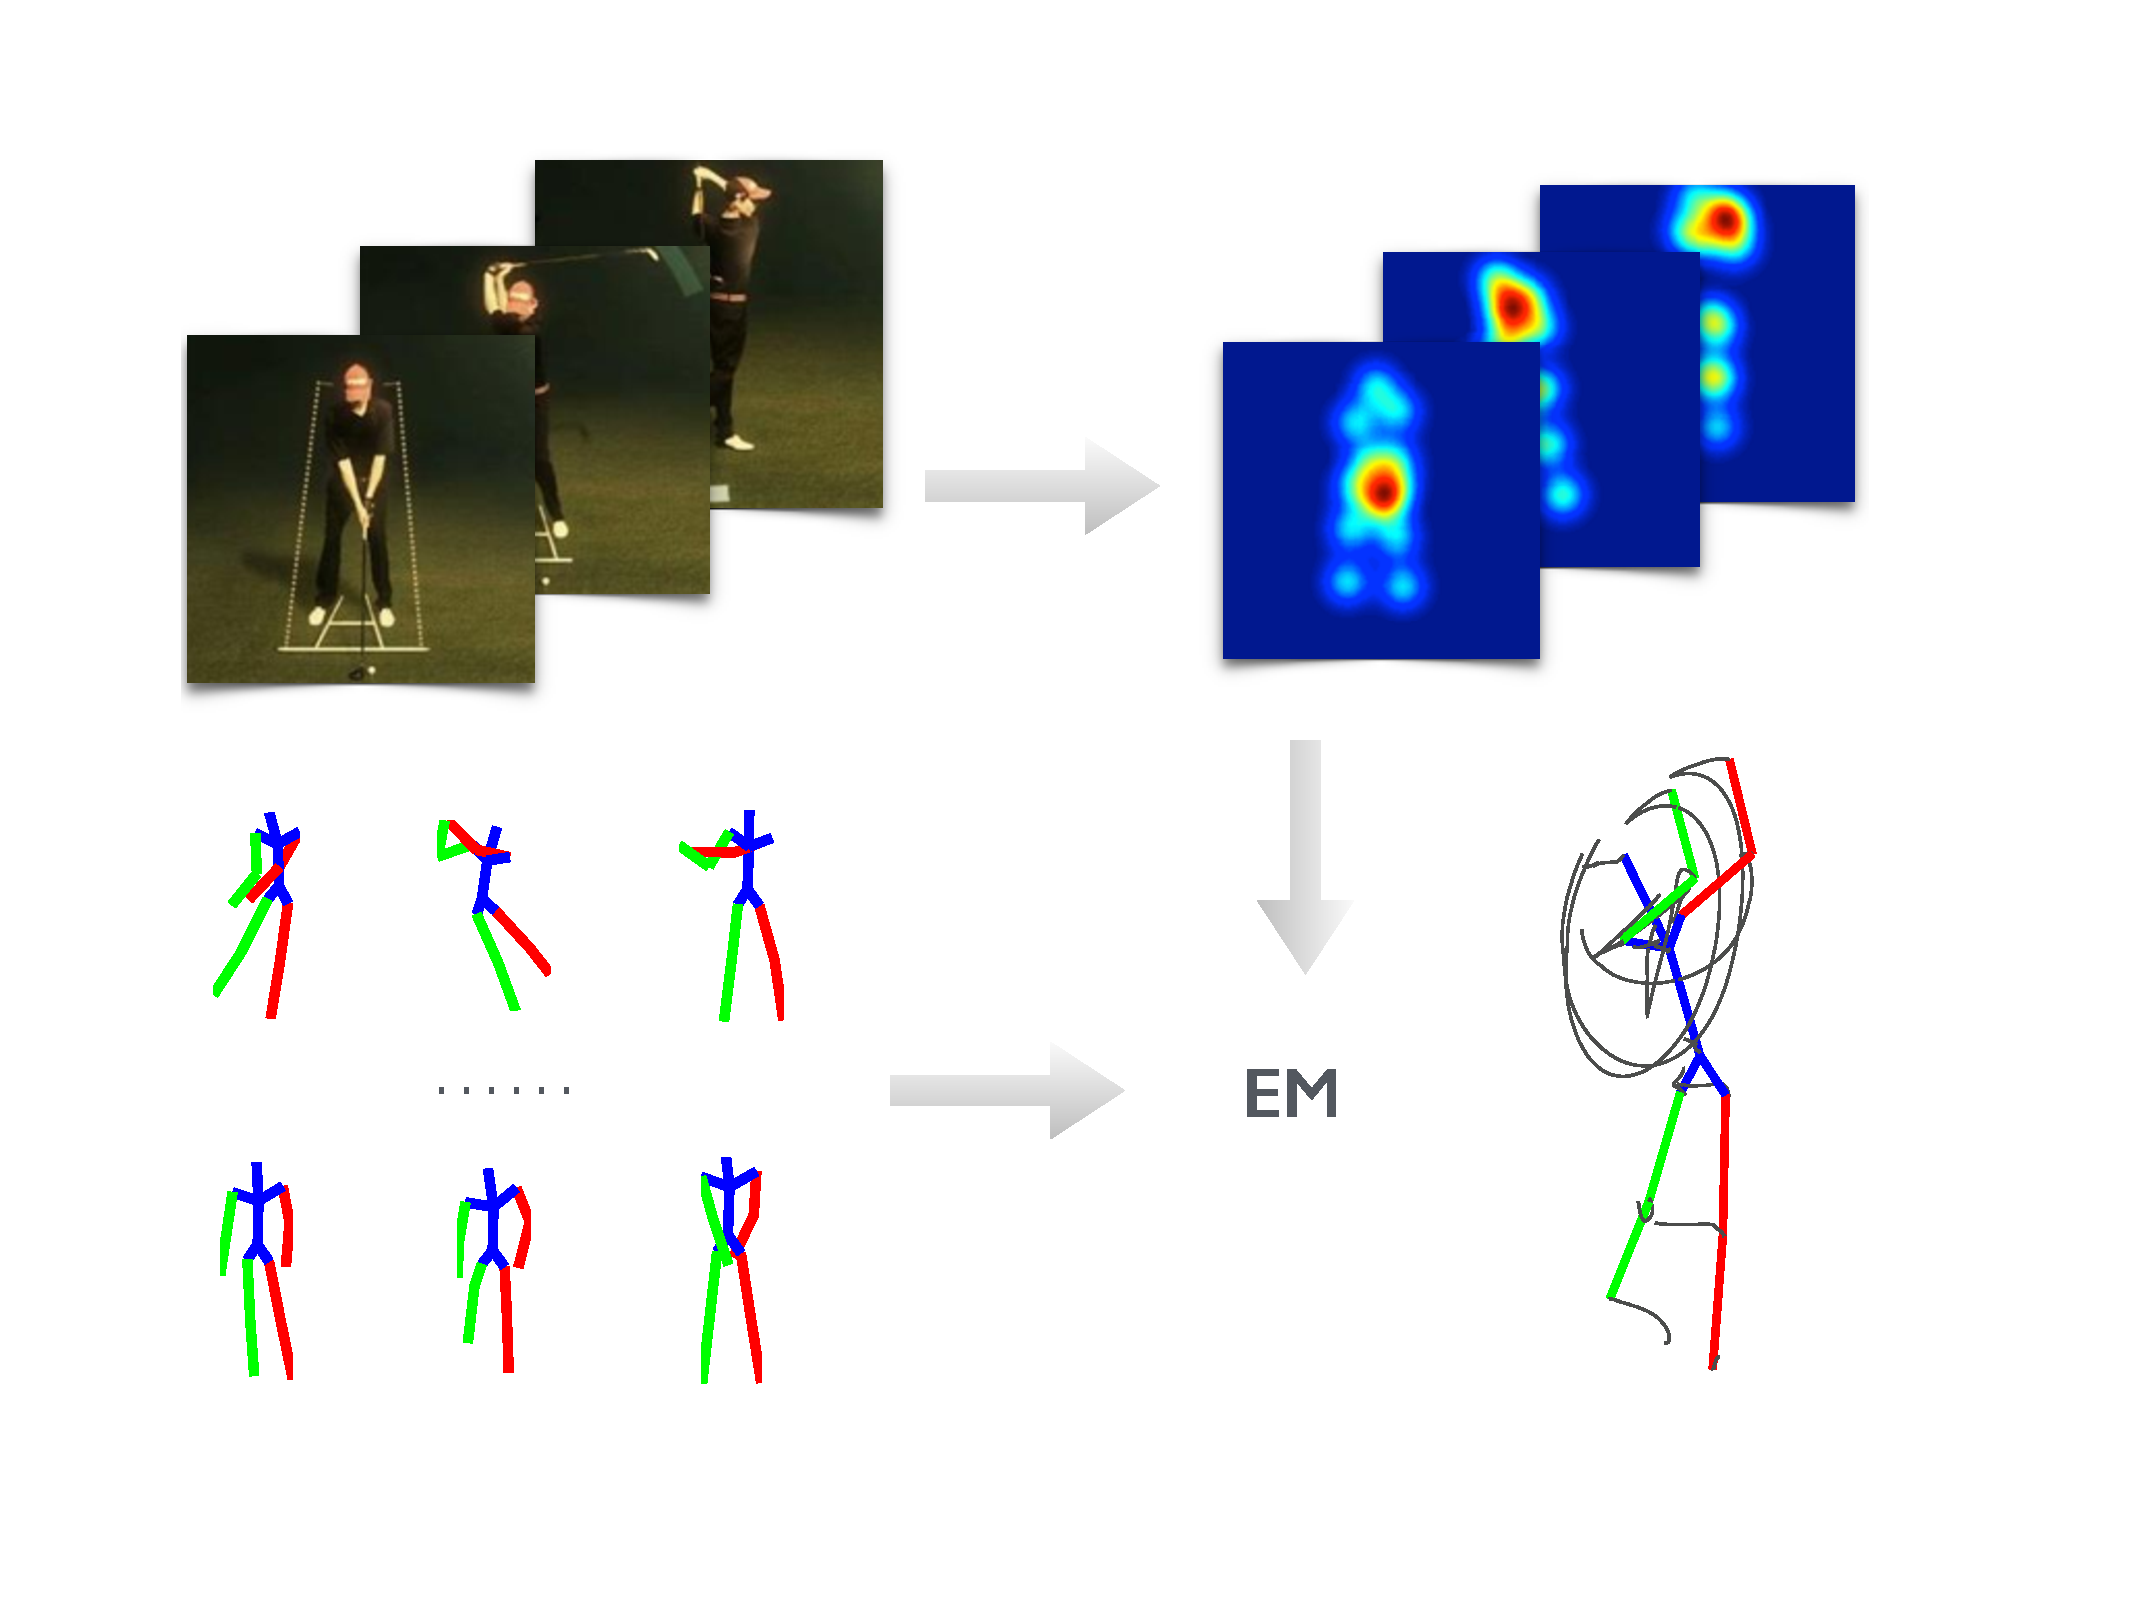
\includegraphics[width=\linewidth]{figures/overview.pdf}
     %\epsfig{file=./figures/spacer.pdf,width=3in}
   \caption{方法总览。(左上) 输入图片序列(右上)基于CNN的2D关节不确定性位置表达。(左下) 3D姿态词典,与(右下) 恢复的3D姿态序列。为了充分考虑不确定性,该问题在概率框架中得到解决,其中2D关节位置被建模为潜在变量并且在EM算法中被边缘化。并且我们还考虑了时间上的平滑性。}
   \label{fig:overview}
   \vspace{-1em}
\end{figure}


本文介绍了一种名为MonoCap的3D人体姿态估计框架,该框架由基于图像的判别式方法和3D重建方法综合组成。
特别地,该方法结合了基于图像的2D部件位置估计和基于模型的3D姿势重建,使得他们可以彼此受益。进一步,为了改善方法对检测器误差、遮挡和重建模糊度的鲁棒性,该方法对3D姿态和相机视角参数进行了时间平滑。
\refFig{fig:overview} 概述了我们的方法。
给定这样这个视频输入 (Fig.\ \ref{fig:overview},左上), 通过一个深度卷积神经网络(CNN),我们可以得到2D关节的热图,它表示了位置的不确定性 (Fig.\ \ref{fig:overview}, 右上). 这些热图使用一个稀疏3D人体模型组合起来 (Fig.\ \ref{fig:overview}, 左下) 通过期望最大(EM)框架,恢复出3D姿态序列。(Fig.\ \ref{fig:overview}, 右下).

